% set packages
\documentclass[11pt,a4paper]{article}
\usepackage{acl2015}
\usepackage{times}
\usepackage{url}
\usepackage{latexsym}

% own packages
\usepackage{graphicx}
\usepackage{placeins}
\usepackage{booktabs}
\usepackage[ngerman]{babel}
\usepackage[utf8]{inputenc}
\usepackage{comment}

\title{The Creation of an hierarchical Category Set as Gold Standard for Letterhead Elements}

\setlength\titlebox{5cm}

\author{First Author \\
  Affiliation / Address line 1 \\
  Affiliation / Address line 2 \\
  Affiliation / Address line 3 \\
  {\tt email@domain} \\\And
  Second Author \\
  Affiliation / Address line 1 \\
  Affiliation / Address line 2 \\
  Affiliation / Address line 3 \\
  {\tt email@domain} \\\And
  Third Author \\
  Affiliation / Address line 1 \\
  Affiliation / Address line 2 \\
  Affiliation / Address line 3 \\
  {\tt email@domain} \\}  
\date{}

\begin{document}
\maketitle

\begin{abstract}
 \input{abstract.tex}
\end{abstract}

\section{Introduction and Motivation}
 \label{sec:Introduction and Motivation}
 \input{section1.tex}


\section{Used Data}
 \label{sec:Used Data}
 The documents, which form the basis of this work, are old authorities correspondences where it comes to the storage of nuclear waste. The topics are mainly plans of emergency measures, eliminating access waters and the closure of individual chambers of the mine. At the beginning there were 71 authorities correspondences. 33 of these documents are freely available online. The remaining 38 documents have been provided as part of a research project. The freely accessible documents were written in the years 2009 to 2013. The others, as far as recognizable, are from the years 1971 to 1975. Although picture elements are included in the OCR output, they aren't used in this work. Twelve of the documents were removed because they effectively did not contain any information content. Thus were still 59 documents left with a total of 1239 text areas. In addition, seven empty text areas were removed. Thus remained in 1232 text areas for the following steps. The resulting in the OCR process documents were available in HTML format and has been brought in a CSV format for the next steps which contains the following information for each text area:


%Die Dokumente, welche die Grundlage dieser Arbeit bilden, sind alte Beh\"ordenkorrespondenzen, in denen sich mit der Lagerung von Atomm\"ull befasst wird. Hierbei geht es um Themen wie zum Beispiel die Planung von Notfallmaßnahmen, Beseitigung von Zutrittswässern und die Schließung einzelner Kammern des Bergwerks. Zu Beginn gab es 71 Beh\"ordenkorrespondenzen. Davon sind 33 Dokumente online frei zugänglich. Die restlichen 38 Dokumente wurden im Rahmen eines Forschungsprojektes zur Verf\"ugung gestellt. Die 33 frei zug\"anglichen Dokumente sind aus den Jahren 2009 bis 2013. Die restlichen 38 Dokumente sind, soweit erkennbar, aus den Jahren 1971 bis 1975. Zwar sind auch Bildelemente in der OCR Ausgabe enthalten, jedoch wird auf diese in dieser Arbeit nicht zur\"uckgegriffen. Es wurden zwölf Dokumente entfernt, da sie effektiv keinen Informationsgehalt enthielten. Somit standen noch 59 Dokumente mit insgesamt 1239 Textbereichen zur Verfügung. Zusätzlich wurden sieben leere Textbereiche entfernt. Somit verblieben für die folgenden Schritte 1232 Textbereiche. Die im OCR Prozess entstandenen Dokumenten lagen im HTML-Format vor und wurden für die weiteren Schritte in einen CSV-Format gebracht der für jeden Textbereich folgende Informationen enthielt: 

\begin{itemize}
\setlength{\itemsep}{-5pt}
 \item Document name and index the text area within the document
 \item identifier of the text area assigned classification
 \item position of the text area in the document and its width
 \item by the OCR process recognized text
\end{itemize}

\begin{comment}
\begin{itemize}
\setlength{\itemsep}{-5pt}
 \item Dokumentenname und Index des Textbereiches innerhalb des Dokumentes
 \item Kennung der dem Textbereich zugewiesenen Klassifikation
 \item Position des Textbereiches im Dokument und seine Breite
 \item der vom OCR-Prozess erkannte Inhalt
\end{itemize}
\end{comment}


\section{Creation of the hierarchical Category Set}
 \label{sec:Creation of the hierarchical Category Set}
 The hierarchical category system extends the seven basic classes, which were used by a project partner for the first classification. The hierarchical structure also offers the possibility that instances of individual classes can be summarized in its superclass. In the following work, the documents were processed by two raters. After careful review of the documents by both raters, five subclasses were added to the first hierarchical category system. Thus, the classification model, which was used for the next steps emerged. To generate the training data each text area of the 59 documents were individually classified by the raters. In order not mutually influence each other in the award of the label, the classification of the two raters was done  independently after a brief discussion about the meaning of each individual classes. In order to verify if and how well the classification matches of both raters, their agreement was calculated by Cohen's Kappa for each evaluation run. In the first evaluation run a $\kappa$ value of 0.6993 was achieved.

%Das hierarchische Kategoriensystem erweitert die sieben grundlegenden Klassen, welche von einem Projektpartner für die erste Klassifikation verwendet wurden. Der hierarchische Aufbau bietet außerdem die Möglichkeit, dass Instanzen einzelner Klassen in ihrer Oberklasse zusammengefasst werden können. Im folgenden Arbeitsverlauf wurden die Dokumente von zwei Bewertern (eng. Rater) bearbeitet. Nach sorgfältiger Durchsicht der Dokumente durch beide Rater wurden dem ersten hierarchischen Kategoriensystem fünf Unterklassen hinzugefügt. Dadurch entstand das Klassifikationsmodell, welches für die nächsten Schritte verwendet wurde. Für die Erzeugung der Trainingsdaten wurde jeder Textbereich der 59 Dokumente einzeln von den Ratern klassifiziert. Um sich nicht gegenseitig bei der Vergabe der Labels zu beeinflussen, wurde diese Klassifikation von beiden Ratern nach einer kurzen Diskussion zum Verständnis der einzelnen Klassen unabhängig voneinander durchgeführt. Um überprüfen zu können, ob und wie gut die Klassifikation der beide Rater übereinstimmt, wurde nach jedem Bewertungsdurchlauf ihre Übereinstimmung durch Cohen's Kappa berechnet. Bereits im ersten Bewertungsdurchlauf wurde ein $\kappa$ Wert von 0,6993 erzielt.

Nevertheless, it became clear that the hierarchical category system was not yet well enough adapted to the available data. Many of the pre-determined classes were not at all or only very rarely assigned. This applies to all subcategories of the third party for example. The third party referred to any personal or address information within a document, which can not be assigned to the actual sender or recipient. There were not only deleted subcategories but also added new ones. This was in the category "(main) text" the case. This was assigned in 41.23 \% of the text areas. Therefore, this category has been split into the two  sub-categories "'content"' and "'structural elements"'.

%Dennoch wurde klar, dass das hierarchische Kategoriensystem noch nicht gut genug an die vorliegenden Daten angepasst war. Viele der vorher festgelegten Klassen wurden gar nicht oder nur sehr selten vergeben. Dies trifft zum Beispiel auf alle Unterkategorien der dritten Partei zu. Die dritte Partei bezeichnet hierbei alle Personen- oder Adressinformationen innerhalb eines Dokumentes, die nicht dem eigentlichen Absender oder Empfänger zugeordnet werden können. Es wurden aber nicht nur Unterkategorien gelöscht, sondern auch neue hinzugefügt. Dies war bei der Kategorie "`(Haupt-)Text"' der Fall. Diese wurde bei 41,23\% der Textbereiche vergeben. Deshalb wurde diese Kategorie in die zwei Unterkategorien "`Fließtext"' und "`Strukturelemente"' aufgespalten. 

The second review cycle revealed that the addition of the two sub-categories "'content"' and "'structural elements"' to the category "'(main) text"' simplifies the assignment of many text areas. Text areas that were assigned as generic "'letterhead element"' (i.e. the root category) because they only contained a single character and were used to structure the text, now can be assigned to the category "'structural element"'. This meant that almost 40 \% of the previously generically as "'letterhead element"' marked text areas could be assigned to another category. Overall, the classification of the raters differed after the second pass on the entire data 324 times. This shows that even before the subsequent merging of the data was an agreement of almost 74 \% and a $\kappa$ 0.7007 from among the raters. Compared to the previous run thus a minimum increase of $\kappa$ is observed. In \newcite{Bakeman1997} is shown that a better value for $\kappa$ is obtained by a larger number of classes. That in this evaluation run now, despite a lower number of classes (37 instead of 47) an increase of $\kappa$ is observed, therefore, indicates a better match of the raters.

%Im zweiten Bewertungsdurchlauf zeigte sich, dass die Ergänzung der zwei Unterkategorien "`Fließtext"' und "`Strukturelemente"' zu der Kategorie "`(Haupt-)Text"' die Zuordnung vieler Textbereiche vereinfacht. Dadurch können nun auch Textbereiche, die vorher nur als generisches "`Briefkopfelement"' (d.h. die Wurzelkategorie) klassifiziert wurden, da sie nur aus einzelnen Zeichen bestanden und zur Auflistung verwendet wurden, jetzt mit der Kategorie "`Strukturelement"' gekennzeichnet werden. Das führte dazu, dass fast 40\% der vorher generisch als "`Briefkopfelement"' gekennzeichneten Textbereiche einer anderen Kategorie zugeordnet werden konnten. Insgesamt unterschied sich die Klassifikation der Rater nach dem 2. Durchlauf auf den ganzen Daten 324 mal. Dies zeigt, dass bereits vor der späteren Zusammenführung der Daten eine Einigung von knapp 74\% und ein $\kappa$ von 0,7007 unter den Ratern bestand. Im Vergleich zum vorherigen Durchlauf ist somit eine minimale Steigerung des $\kappa$ zu beobachten. In \newcite{Bakeman1997} wird gezeigt, dass durch eine größere Anzahl an Klassen ein besserer Wert für $\kappa$ erreicht wird. Dass in diesem Bewertungsdurchlauf nun trotz einer geringeren Anzahl von Klassen (37 anstatt 47) eine Steigerung von $\kappa$ beobachtet wird, weist daher auf eine bessere Übereinstimmung der Rater hin.

In order to create a unique category assignment for this data on the basis of the final hierarchical category system, the text areas whose assignments were different in the two raters, were checked again together and a category was chosen. Overall, the decisions, which of the two views was followed out very evenly distributed. On the results of the merge you can see that only the upper categories of the category system were not assigned. It follows that is at least one example of the training data available for each of the categories.

%Um eine eindeutige Kategorienzuweisung für die vorliegenden Daten auf Grundlage des finalen hierarchischen Kategoriensystem erzeugen zu können, wurden die Textbereiche, deren Zuweisungen sich bei den beiden Ratern unterschieden, zusammen noch einmal überprüft und dabei über eine Einigung diskutiert. Oftmals wurde hierbei die Auffassung eines der beiden Rater übernommen. Insgesamt sind die Entscheidungen, welcher der beiden Auffassungen gefolgt wurde, sehr gleich verteilt ausgefallen. An den Ergebnissen der Zusammenführung (eng. Merging) sieht man, dass nur Oberkategorien des Kategoriensystems nicht vergeben wurden. Daraus folgt, dass für jedes der Blätter mindestens ein Beispiel für die Trainingsdaten zur Verfügung steht. Von den 27 Blattkategorien sind somit nur neun mit unter zehn Beispielen vertreten. 



\section{Classification Experiments}
 \label{sec:Classification Experiments}
 %Um zu überprüfen, ob die manuell vergebenen Klasse auf den Trainingsdaten maschinell reproduziert werden können, wurde auf eine Implementierung gängiger Klassifikationsalgorithmen aus einer früheren Arbeit \cite{Pressler2014} in dem oben erwähnten Forschungsprojekt zurückgegriffen. Die auf der $MALLET$ Toolbox \cite{McCallum2002} basierende Implementation wurde auf das im Rahmen der vorliegenden Arbeit entwickelte hierarchische Kategoriensystem übertragen, optimiert und erweitert. In Preßler \cite{Pressler2014} wurden bereits gute Ergebnisse für die Accuracy erzielt, die im Bereich von 0.8 bis 0.9 liegen. Diese variieren je nach verwendetem Verfahren. Bei dieser Klassifikation wurden aber über 85\% der Textbereiche den Kategorien "`Sonstiges"' (47\%) und "`Inhalt"' (39\%) zugeordnet und die restlichen Klassen teilweise gar nicht erkannt. Durch die Verwendung des hierarchischen Kategoriensystems soll überprüft werden, ob zusätzliche Informationen durch eine verbesserte Gliederung der Kategorien erhalten werden können, ohne dabei große Verluste bei der Präzision (eng. Accuracy) der Klassifikatoren hinnehmen zu müssen. Neben der Accuracy wurde zusätzlich für jede Kategorie die Genauigkeit (eng. Precision), die Trefferquote (eng. Recall) und der sich daraus ergebende F1 Wert berechnet.

%Für den Trainingsalgorithmus wurde das auf Java basierende $MALLET$ verwendet. Die für die Klassifikation verwendeten Trainingsalgorithmen sind Naive Bayes, Winnow und Balanced Winnow, Maximum Entropy und Entscheidungsbäume. Auf die Verwendung des in der vorausgehenden Arbeit \cite{Pressler2014} verwendeten C4.5 Klassifikators wurde in den weiteren Arbeitsschritten verzichtet, da das Trainings aller Klassifikatoren im Vergleich zum Training der Klassifikatoren ohne den C4.5 Klassifikator 27 mal länger dauerte, ohne dabei bessere Ergebnisse zu erzielen. 

%Für die ersten Experimente mit überwachter Klassifikation wurde auf die selben Trainingsalgorithmen zurückgegriffen, die bereits in Preßler \cite{Pressler2014} verwendet wurden. Als Trainingsdaten wurden hierbei die Daten verwendet, welche durch die Einigung der beiden Rater entstanden sind (vgl. Abschnitt \ref{subsec:Ergebnisse nach dem Merging}).

%Da innerhalb dieser Trainingsdaten einige Klassen häufig mehrmals hintereinander vergeben wurden und die Implementation die Teilmengen für die k-fold Cross-Validation anhand ihres Index zusammenfügt, wurden die vorliegenden Daten in eine zufällige Reihenfolge gebracht, um eine bessere Verteilung der einzelnen Testfälle in den Trainingsdaten zu gewährleisten. Die ersten Testergebnisse zeigen, dass durch Klasssifikatoren wie den Maximum Entropie Klassifikator oder den Balanced Winnow Klassifikator bereits gute Werte in der Accuracy im Bereich von 0.7 erzielt werden. 

%Wie bereits in Abschnitt \ref{subsec:Verwendete Verfahren} erwähnt, erreichte der C4.5 Klassifikator trotz seiner längeren Laufzeit lediglich einen Accuracy Wert der unter dem Durchschnitt der restlichen Klassifikatoren liegt. Auch die Decision Tree und Winnow Klassifikatoren erzielten unbefriedigende Werte, weshalb im weiteren Verlauf nur auf den Naive Bayes Klassifikator, Maximum Entropie und Maximum Entropie L1 Klassifikator und den Balanced Winnow Klassifikator eingegangen wird.

%Um jedoch genauere Aussagen über die Güte eines Klassifikators im Hinblick auf einzelne Klassen zu erhalten, wurden zusätzlich zur Accuracy jedes Klassifikators noch die Precision und Recall Werte jeder einzelnen Klasse durch eine Erweiterung der bestehenden Implementation berechnet. % Bei der Cross-Validation erfolgt die Aggregation oft über das Summieren der Precision und Recall Werte für die einzelnen Durchläufe und eine Mittelwertbildung über denselben. Zunächst wurde dieses Verfahren durch die Verwendung der Trail Klasse von $MALLET$ implementiert. Hierbei wurden die getF1(), getPrecision() und getRecall() Methoden verwendet. Da ein Trial im Verfahren der 10-fold Cross-Validation jedoch durch einen Split der Daten in neun Trainings- und einen Testdatensatz erzeugt wird, besteht ein Testdatensatz nur aus 132 oder 133 Textbereichen. Das hierarchisches Kategoriensystem besteht aber bereits aus 37 Klassen, wovon 32 im Rahmen der Trainingsdatenerzeugung vergeben wurden. Da die Klassen innerhalb des Trainingskorpus nicht gleichmäßig verteilt sind, ist ein Vorkommen jeder Klasse in jedem Datensatz sehr unwahrscheinlich. Darüber hinaus existieren Klassen, die sogar weniger als 10 mal vergeben wurden und folglich nicht in jedem Datensatz vorkommen können.

%Dies hatte zur Folge, dass die Methoden für nicht vorhandene Klassen in den Testdaten den Wert 1 für Precision und Recall lieferten. Logisch gesehen sind diese Werte zwar zu rechtfertigen, da der Klassifikator null von null Beispielen gefunden hat, führen aber bei der Aggregation der einzelnen Daten, welche aus den verschiedenen Trials gewonnen wurden, zu einer Verzerrung des Gesamtergebnisses. Die Ergebnisse für seltener vorkommende Klassen werden dadurch irreführenderweise dem Wert 1 angenähert. Erst ab einem totalem Vorkommen einer Klasse in den Gesamtdaten von 20 bis 25 werden realistische Werte erzielt. Auch zeigte sich, dass der durch die Methode getF1() erhaltene F1 Wert oftmals von dem Wert abweicht, welcher aus den Precision und Recall Werten nach Formel \ref{eq:Berechnung F1} (vgl. Seite \pageref{eq:Berechnung F1}) berechnet werden kann. Um verlässliche und in sich stimmige Ergebnisse zu erzielen, wurde daher auf die Verwendung der getF1(), getPrecision() und getRecall() Methoden verzichtet. 

% Stattdesssen wurde in der vorliegenden Arbeit die Aggregation über das Summieren der Confusionmatrizen der einzelnen Validierungsläufe, welche durch die Verwendung der ConfusionMatrix Klasse von $MALLET$ erzeugt wurden, zu einer Gesamtmatrix vorgenommen. Die Werte für F1, Precision und Recall wurden auf Basis dieser Gesamtmatrix berechnet. 

% Eine stichprobenartige Überprüfung zeigte, dass zahlenmäßig häufig auftretende Klassen wie zum Beispiel "`Fließtext"' (1421) oder "`Sender(Adresse, Postfach"' (1123) eine geringe Abweichung der F1 Werte von wenigen Prozentpunkten (im Bereich von circa plus zwei bis minus sechs Prozent) von den mittels getPrecision() und getRecall() berechneten F1 Werten aufweisen. Dabei besitzen die durch die Aggregation der Confusionmatrizen berechneten F1 Werte, in der Regel, den geringeren Wert. Das hat den positiven Nebeneffekt, dass die Leistungsfähigkeit unserer Klassifikatoren eher unterschätzt als überschätzt wird. Dieser positive Aspekt ist auch bei zahlenmäßig selten auftretenden Klassen wie zum Beispiel "`Datum"' (121) oder "`Ort"' (13) zu beobachten.

% Bei diesen Klassen werden durch die Verwendung der getPrecision() und getRecall() Methoden unrealistisch hohe F1 Werte auf Grund von logischen Werten im Bereich von beinahe 0.9 erzielt, welche durch die Aggregation über die Confusionmatrizen vermieden werden.

In order to evaluate whether the manually assigned classes to the training data can be reproduced automatically, we employed several machine learning algorithms and compared their performance. In a first set of experiments we used a standard bag of words model. As classes within the training data were often assigned repeatedly, the order of the text blocks in our gold standard was randomized to create a better distribution of the individual test cases in the training data. To make the best use of our limited amount of data, we used ten-fold cross-validation for training and testing.

Among the range of classifiers we initially trained were standard Naive Bayes, Maximum Entropy (with and without regularisation), Winnow, Balanced Winnow and two decision tree learners (modified ID3 and C4.5).\footnote{For the implementation of the training algorithms we used the java based $MALLET$ toolkit. Cf.\ \url{http://mallet.cs.umass.edu}.}

An initial run of experiments on our annotated data set using the full category hierarchy (Fig.\ \ref{fig:letterexample}) showed that accuracy values in the range of 0.7 can be achieved by a Maximum Entropy classifier (using L1 regularisation) and a Balanced Winnow classifier. We decided not to pursue further with (unbalanced) Winnow and the decision tree classifiers as they achieved low accuracy values despite far longer training times in some cases (Table \ref{tab:accuracy}).


\begin{table}
 \centering
 \begin{tabular}{l c}
  \toprule
  \textbf{Classifier} & \textbf{Accuracy} \\
  \midrule
  Naive Bayes			& 0.636	\\
  Maximum Entropie		& 0.708 \\ 
  Maximum Entropie L1	& 0.689	\\	
  Winnow				& 0.496	\\
  Balanced Winnow		& 0.687	\\
  Decision Tree			& 0.378 \\
  C4.5					& 0.558	\\
  \bottomrule
 \end{tabular}
 \caption{Accuracy values achieved by various supervised learning algorithms on our annotated training data (using the complete hierarchy and 10-fold cross-validation)}
 \label{tab:accuracy}
\end{table}


%%%%%%%%%%%%%%%%%
% Table tab:accuracy caption
% Accuracy values achieved by various supervised learning algorithms on our annotated training data (using the complete hierarchy and 10-fold cross-validation).
%%%%%%%%%%%%%%%%%

To obtain more accurate information about the performance of classifiers with regard to individual classes, we calculated precision, recall and F1 values for each class. Here we noticed, that despite reasonable accuracy values, the classifiers achieved F1 values of less than 0.5 for between a third (34.4\%) and nearly two thirds (62.5\%) of classes in classes in our category system. Unsurprisingly this often happened for classes which had very few example instances in our training data. In designing the category hierarchy and compiling our gold standard annotation we were mostly driven by the idea of a robust and versatile classification framework for our chosen domain and a body of ``ground truth'' in the sense of that framework and not so much by practical considerations of how well the data could serve as a training set for supervised learning. As a result we decided to keep some of the classes in our category hierarchy which were used less than ten times in our annotated data, if we felt that the category was useful in principle.

In practice we found that classes with less than 25 occurrences overall in our data set were poorly recognized. An exception to this are ``generic salutation'' and ``salutation, name'' which had precision and recall values in excess of 90\% for all classifiers despite occurring only 11 and 8 times respectively. This may be due to the formulaic nature of the corresponding text.

% hierarchisches kategoriensystem

In addition to comparing classifiers trained on various truncations of the category hierarchy, we experimented with the introduction of additional features which go beyond a pure bag of words model. In our approach we introduced one additional feature for each word in the bag of words which was intended to capture the capitalisation signature of the word. This was done by including a string of upper and/or lower case xs in the bag corresponding to the upper and lower case letters in the original word. Thus the word ``Bundesamt'' would be transformed into ``Xxxxxxxxx''.

% In addition to evaluating different classifiers against each other, we varied our experiments along two different lines.

\vspace*{2cm}

% As for classifiers, after some experiments we decided to use Naive Bayes, Maximum Entropy, Maximum Entropy L1, and Balanced Winnow classifiers. We also trained Winnow, C4.5 and Decision Trees classifier at the beginning, but omitted those in the further steps because they either achieved a way lower accuracy or needed a far longer training time (about 27x) without better results.  

% The first test results show that good results in accuracy in the range of 0.7 already can be achieved by the maximum entropy L1 classifier as well as the balanced winnow classifier. However, to obtain more accurate information about the quality of a classifier with regard to individual classes, we calculated the precision and recall values of each class by extending the existing implementation. 
%bene vorher schon genannt? auf die confusion matrix eingehen?

% After calculating the precision and recall values we noticed, although we achieved accuracy values around 0.7, that the classifiers achieved bad precision and recall values under 0.5 for 34.4 to 62.5 \% of the classes. 


\vspace*{2cm}

% Bei der Verwendung des hierarchischen Kategoriensystems zeigte sich bereits, dass trotz der relativ guten Accuracy manche der Klassen sehr schlechte Werte bezüglich Precision und Recall aufweisen. Dies tritt sehr häufig bei Klassen mit geringem Vorkommen auf. Auch wird deutlich, dass der Naive Bayes Klassifikator die meisten Probleme mit der geringen Anzahl von Trainingsbeispielen hat. Grundsätzlich wird aber auch klar, dass Klassen die insgesamt weniger als 25 mal im Trainingsdatensatz vorkommen häufig schlecht erkannt werden. Diese Grenze fiel bereits bei der Verwendung der getPrecision() und getRecall() Methoden von $MALLET$ auf (s.o.). Eine Ausnahme hierzu bilden die Klassen "`Generische Begrüßung"' und "`Begrüßung, Name"'. Obwohl sie nur 11 bzw. 8 mal vorkommen, besitzen sie bei allen vier Klassifikatoren hohe Werte für Precision und Recall die im Bereich von 0.9 bis 1.0 liegen. Auch haben manche Klassen zwar eine hohe Precision aber einen sehr geringen Recall. 

%Dies tritt hauptsächlich bei Klassen wie "`Sendeweg"', "`Anhangzeile"' und "`Sender, Empfänger"' auf, welche nur ein geringes Vorkommen aufweisen. 

Beim Vergleich der einzelnen Klassifikatoren wird deutlich, dass der Naive Bayes Klassifikator die meisten Probleme mit den vorliegenden Daten hat. Sein Accuracy Wert liegt 0.05 bis 0.07 unter dem der Anderen. Während die restlichen drei Klassifikatoren für sechs oder sieben Klassen einen F1 Wert von null erreichten, war dies beim Naive Bayes Klassifikator bei 13 Klassen der Fall. Das heißt für 13 zugegebenermaßen geringfügig vorkommenden Klassen der insgesamt 32 vergebenen Klassen leistet der von uns trainierte Naive Bayes Klassifikator effektiv nichts. Auch bei den restlichen Klassen erzielte der Naive Bayes Klassifikator meistens schlechtere Ergebnisse. Ausnahmen hierbei bilden lediglich die Klassen "`Briefkopfelement"' und "`Sender (Telefon/Fax)"'. Für die Klasse "`Sender (Email/Webseite)"' erreichte nur der Maximum Entropie L1 Klassifikator einen besseren Wert als der Naive Bayes Klassifikator. 

Beim weiteren Vergleich der Klassifikatoren fällt auf, dass der Balanced Winnow Klassifikator als einziger einen Wert größer als null für die Klasse "`Datum etc."' erzielt. Trotz eines geringen Vorkommens von nur fünf Textbereichen in den Trainingsdaten liegt der F1 Wert des Balanced Winnow Klassifikators für diese Klasse bei 0.889. Alle Ergebnisse der einzelnen Klassifikatoren dieses Durchganges sind in den Tabellen \ref{tab:NaiveBayes 4Ebenen} bis \ref{tab:BalancedWinnow 4Ebenen} in den Anlagen aufgelistet.

Wie bereits in Abschnitt \ref{subsec:Hierarchisches Kategoriensystem} beschrieben, besteht ein Vorteil eines hierarchischen Kategoriensystems darin, dass jede Instanz jeder Klasse auch zu jeder Oberklasse der betreffenden Klasse gehört. Dadurch können Klassen mit einem geringen Vorkommen zu ihrer Oberklasse hinzugefügt werden, ohne die intensionale Definition der Klasse wesentlich zu verändern. Diese Eigenschaft ermöglicht es, durch die Abwandlung des bestehenden hierarchischen Kategoriensystems Trainingsdatensätze mit abgewandelten Klassenlabeln zu erzeugen. In unserem Fall wurden drei weitere Versionen der Trainingsdatensätze durch das Kollabieren des Kategoriensystems auf drei Ebenen, zwei Ebenen und eine ebenenunabhänige Version erzeugt, bei der jede Klasse, deren Vorkommen im Trainingsdatensatz geringer als 19 war, in ihre Oberklasse gemappt wurde. Die Grenze von 19 stellt dabei den Median der Klassenstärken dar, also den Median der Anzahlen der den verschiedenen Klassen zugeordneten Textbereichen in den Trainingsdaten (diese letzte Version wird im weiteren Verlauf dieser Arbeit der Einfachheit halber als Median Version bezeichnet). Durch dieses Verfahren wird überprüft, inwiefern die Werte für Precision und Recall der einzelnen Klassen sich durch die zusätzlichen Elemente verändern. Grundsätzlich wird davon ausgegangen, dass sich der Accuracy Wert durch die geringere Anzahl von Klassen verbessert, da bei der Klassifikation zwischen weniger Klassen unterschieden werden muss. Das Verhalten von Precision und Recall ist hierbei schwer einzuschätzen, da bei einer größeren Anzahl von Trainingsbeispielen einerseits davon auszugehen ist, dass sich Precision und Recall verbessern. Jedoch können die zusätzlichen Elemente auch dazu führen, dass die charakteristischen Merkmale der Klasse nicht mehr so stark ausgeprägt sind, da die zusätzlichen Elemente von den Ursprünglichen abweichen. In Abbildung \ref{pic:Accuracy_ohneX_mitX} wird gezeigt, dass sich für das normale Mapping pro Ebene die Accuracy Werte für jeden Klassifikator verbessern. Überraschenderweise fällt bei der Betrachtung der Accuracy Werte auf, dass bei der Verwendung des Median gemappten hierarchischen Kategoriensystems, welches deutlich weniger Klassen enthält als das normale hierarchische Kategoriensystem, kaum eine Steigerung erreicht wird. Der Accuracy Wert für Balanced Winnow sinkt sogar im Vergleich zum Ausgangswert. 

Zusätzlichen zu den verschiedenen Versionen des hierarchischen Kategoriensystems wurde ein Verfahren verwendet, welches bereits in Preßler \cite{Pressler2014} zur Anwendung kam. Hierbei werden für jeden Textbereich zusätzliche Features (im folgenden X-Features genannt) seinem Inhalt entsprechend hinzugefügt. Der Aufbau dieser zusätzlichen Features ist abhängig von den bereits enthaltenen Features eines Textbereiches. Für jedes Element des Textbereiches (d.h. im wesentlichen für jedes enthaltene Wort) wird ein zusätzliches Element hinzugefügt. Somit verdoppelt sich die Anzahl der Features pro Textbereich. Die Form der zusätzlichen Features ergibt sich aus daraus, dass zwischen Wörtern bzw. Zeichen und Zahlen differenziert wird. Wörter werden zusätzlich durch ihre Groß- und Kleinbuchstaben unterschieden. Ein großes X im zusätzlichen Element steht hierbei für einen Großbuchstaben. Analog hierzu steht ein kleines x für einen kleinen Buchstaben. Somit ergibt sich für das Wort "`Bundesamt"' die Zeichenkette "`Xxxxxxxxx"'. Zahlen werden hierbei etwas anders behandelt. Sie beginnen mit einem großen X gefolgt von einer Anzahl von großen N, welcher der Länge der Zahl entspricht. Somit ergibt sich für die Zahl "`53175"' die Zeichenkette "`XNNNNN"'. Diese Konvention wurde bereits in Preßler \cite{Pressler2014} verwendet. Das Ziel dieser zusätzlichen Features besteht darin, Wörter oder Zahlen die ein ähnliches Format besitzen (beispielsweise Postleitzahlen) stärker miteinander in Verbindung zu bringen als dies durch die nominelle Inklusion der ursprünglichen Zeichenkette als Features in einem Bag-of-Words Modell geschehen kann. Möglicherweise können die Klassifikationsergebnisse dadurch verbessert werden. In der vorangehenden Arbeit zeigte sich allerdings, dass die Verwendung dieser X-Features nicht den gewünschten positiven Effekt erzielte. Die meisten Klassifikatoren reagierten in Preßler \cite{Pressler2014} eher mit einer schlechteren Accuracy als zuvor. Eine geringe Verbesserungen der Accuracy konnte lediglich bei den Maximum Entropie L1, Decision Tree und C4.5 Klassifikatoren gemessen werden. Um zu überprüfen, ob durch die Verwendung der X-Features auf unserem Datensatz eine Verbesserung der Ergebnisse der Klassifikatoren erreicht werden kann, wurden die Trainingsalgorithmen auf einer Kopie des zuvor verwendeten Datensatzes, welcher die zusätzlichen X-Features enthält, trainiert. Dabei zeigte sich, dass die Accuracy des Naive Bayes Klassifikator um bis zu 0.07 sinkt. Dies überrascht nicht, da dieser Klassifikator, wie bereits in Abschnitt \ref{subsubsec:Naive Bayes Klassifikator} beschrieben, schlecht mit ähnlichen Features umgehen kann. Die Auswirkung auf die anderen Klassifikatoren ist nicht so schwerwiegend. Beim Maximum Entropie Klassifikator wurde durch die Verwendung der X-Features in drei von vier Fällen eine Verbesserung der Accuracy von bis zu 0.014 festgestellt. Lediglich unter Verwendung des Kategoriensystems mit 2 Ebenen wurde ein minimal geringerer Wert erzielt (0.856 ohne X-Features und 0.852 mit X-Features). Für den Maximum Entropie L1 Klassifikator fallen die Ergebnisse hierbei ähnlich aus. In zwei von vier Fällen verbesserte sich die Accuracy, während sich bei den anderen entweder kein oder nur ein sehr geringer Verlust bemerkbar machte. Ein anderes Ergebnis kann man beim Balanced Winnow Klassifikator beobachten. Dieser erreichte ohne die X-Features in drei von vier Fällen ein minimal besseres Ergebnis als mit ihnen. Grundsätzlich lässt sich sagen, dass in den meisten Fällen die Verwendung der X-Features kaum merkliche Unterschiede erzeugt. Die Unterschiede in den Accuracy Werten sind in Tabelle \ref{tab:Accuracy Klassifikation} zusammengefasst.


Bei der Betrachtung des Verhaltens der Klassifikatoren unter Verwendung der reduzierten Kategoriensysteme fällt beim Naive Bayes Klassifikator auf, dass die Ergebnisse für Sender und Empfänger sehr unterschiedlich ausfallen. Die Klassen des Senders werden einzeln meistens besser klassifiziert als wenn man sie in eine Klasse zusammenfügt. Beim Empfänger ist das umgekehrt. Für diese Klasse wurden die besten Ergebnisse erzielt, wenn man sie zu einer Klasse zusammenfügt. Diese Beobachtung kann man auch bei den anderen Klassifikatoren machen. Die einzige Ausnahme hierzu stellt der Maximum Entropie L1 Klassifikator dar. Mit ihm werden für alle Empfängerklassen ähnlich gute und teils auch bessere Ergebnisse für den F1 Wert erzielt (außer für "`Empfänger(Telefon/Fax)"', was aber durch das totale Vorkommen der Klasse von eins im Datensatz irrelevant ist).

Auch fällt auf, dass 19 der 32 vergebenen Klassen im hierarchischen Kategoriensystem mit vier Ebenen weniger als 20 mal in unserem Datensatz vergeben wurden. Um nachvollziehen zu können, wie sehr sich die Anzahl einer Klasse innerhalb der Trainingsdaten auf den F1 Wert auswirkt, wurde in dieser Arbeit für jeden Klassifikator überprüft, wie oft ein Klassifikator einen niedrigen F1 Wert für selten vorkommende Klassen erzielt. Im Vergleich dazu wurde auch überprüft, wie oft dieser Klassifikator einen niedrigen F1 Wert für häufig vorkommende Klassen erzielt. Für das Vorkommen wird eine Grenze von 20 verwendet, da sich die Grenze von 20 bis 25 bereits in früheren Arbeitsschritten dieser Arbeit bemerkbar machte. Es wird deutlich, dass für Klassen, die häufiger als 20 mal im Datensatz vorkommen, deutlich häufiger ein F1 Wert über 0.5 erzielt wird als für Klassen die seltener als 20 mal vorkommen. Auch sieht man, dass der Maximum Entropie L1 und der Balanced Winnow Klassifikator deutlich häufiger F1 Werte über 0.5 bei einer geringen Anzahl von Trainingsbeispielen erzielen als die anderen zwei Klassifikatoren. Die Ergebnisse sind in Tabelle \ref{tab:Vergleich Accuracy Vorkommen 4Ebenen} und Tabelle \ref{tab:Vergleich Accuracy Vorkommen 3Ebenen} bis \ref{tab:Vergleich Accuracy Vorkommen Median} dargestellt. Für eine detailliertere Darstellung aller Ergebnisse jedes einzelnen Klassifikators wurden die genauen Ergebnisse für F1, Precision und Recall für jede Klasse in Tabelle \ref{tab:NaiveBayes 4Ebenen} bis \ref{tab:BalancedWinnow Median xFeatures} aufgelistet.

%\begin{tabular}{l l  l l l l}
%\toprule
%		&			& {\bf Naive Bayes} & {\bf Max Ent} & {\bf Max Ent L1} 	& {\bf B Winnow}	\\
%\cmidrule{3-6}
%Category& Apperance & Acc: 0.636		& Acc: 0.708	& Acc: 0.689		& Acc:				\\
%\midrule
%1122	& 19		& 0.182				& 0.647			& 					&					\\
%1123	& 68		& 0.634				& 0.782			& 0.712				&					\\
%1132	& 10		& 0.000				& 0.462			&					&					\\
%1133	& 49		& 0.477				& 0.571			& 0.552				&					\\
%141		& 60		& 0.294				& 0.609			&					&					\\
%1421	& 330		& 0.813				& 0.867			&					&					\\
%1612	& 8			& 0.933				& 0.933			&					&					\\
%162		& 41		& 0.833				& 0.895			&					&					\\
%\bottomrule
%\end{tabular}



\section{Future Work}
 \label{sec:Future Work}
 \input{section5.tex}

\section*{Acknowledgments}
 \input{acknowledgments.tex}
 
 
% include your own bib file like this:
%\bibliographystyle{acl}
%\bibliography{acl2015}

\begin{thebibliography}{}

 \bibitem[\protect\citename{{Bakeman et al.}}1997]{Bakeman1997}
Bakeman, R., Quera, V., McArthur, D. und Robinson, B. F.: {\em Detecting Sequential Patterns and Determining Their Reliability With Fallible Observers}, in: {\em Psychological Methods}, Vol. 2, S. 357--370, 1997. 



\bibitem[\protect\citename{{Autoren}}Jahr]{Kennung im Text}
{Autoren, erster Vorname ausgeschrieben restlichen mit . Personen mit , getrennt}.
\newblock Jahr.
\newblock {\em Titel}.
\begin{comment}
italic text:
Titel nur bei Büchern,
Artikel der Journal Name,
Workshop
Abschnitt in einem Buch nicht italic
\end{comment}
\newblock Verlag, Verlagsort, Verlagsland.
\newblock Volume(Item/Number):Seitevon-bis. 
\begin{comment}
	Volume durchlaufend 
	Number jahrbezogen
\end{comment}
\end{thebibliography}

\newpage 
\begin{figure}
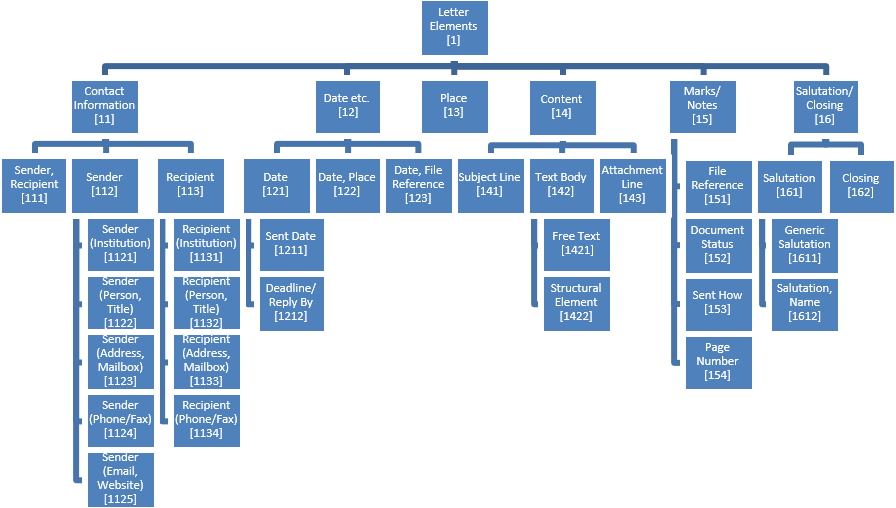
\includegraphics[scale=0.4]{hKat.png}
\end{figure}


\end{document}
